\chapter{Introducción}
\section{Descripción del proyecto}
\subsection{Antecedentes}
Incluya en esta sección una reseña histórica del proyecto 
\subsection{Objetivos}
Liste los objetivos del proyecto.
\begin{itemize}
    \item \textbf{Objetivo General}
    \begin{itemize}
        \item Objetivo general del proyecto redactado con un verbo infinitivo. Debe cubrir las generalidades del proyecto
    \end{itemize}
    \item \textbf{Objetivos Específicos}
    \begin{itemize}
        \item Objetivos específicos con mayor nivel de detalle
        \item Normalmente los objetivos específicos hacen referencia a "módulos" del sistema
    \end{itemize}
\end{itemize}
\section{Datos gerenciales del proyecto}
\subsection{Acta Constitutiva del proyecto}
Lorem ipsum dolor sit amet, consectetur adipiscing elit. Nunc sed cursus dolor. Aliquam mi ipsum, ullamcorper ac tellus iaculis, interdum egestas orci. In vitae leo in tellus feugiat interdum.

\subsection{Interesados}
Liste los diferentes involucrados en este proyecto, incluya en una figura un organigrama del equipo de trabajo.

Lorem ipsum dolor sit amet, consectetur adipiscing elit. Nunc sed cursus dolor. Aliquam mi ipsum, ullamcorper ac tellus iaculis, interdum egestas orci. In vitae leo in tellus feugiat interdum.


\begin{figure}[H]
  \centering
    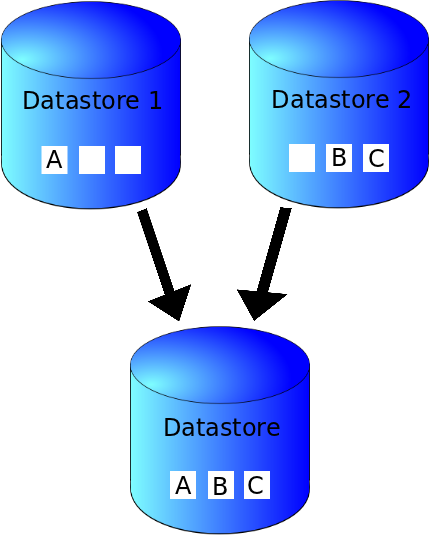
\includegraphics[height= 10cm, width=15cm]{project/images/data-sync}
  \caption{\textbf{IMAGE CAPTION}}
\end{figure}

